\documentclass[../main.tex]{subfiles}


%opening
\maketitle
According to the results in Aiyagari(1994), the differences between the saving rates with an without insurance are quite small for moderate and empirically plausible values of $\sigma$, $\rho$, and $\mu$. However for high values of $\sigma$, $\rho$, and $\mu$, the presence of idiosyncratic risk can raise the saving rate quite significantly. \\

The table below is extracted from Aiyagari(1994) and clearly shows this point. 

\begin{figure}[H]
\centering
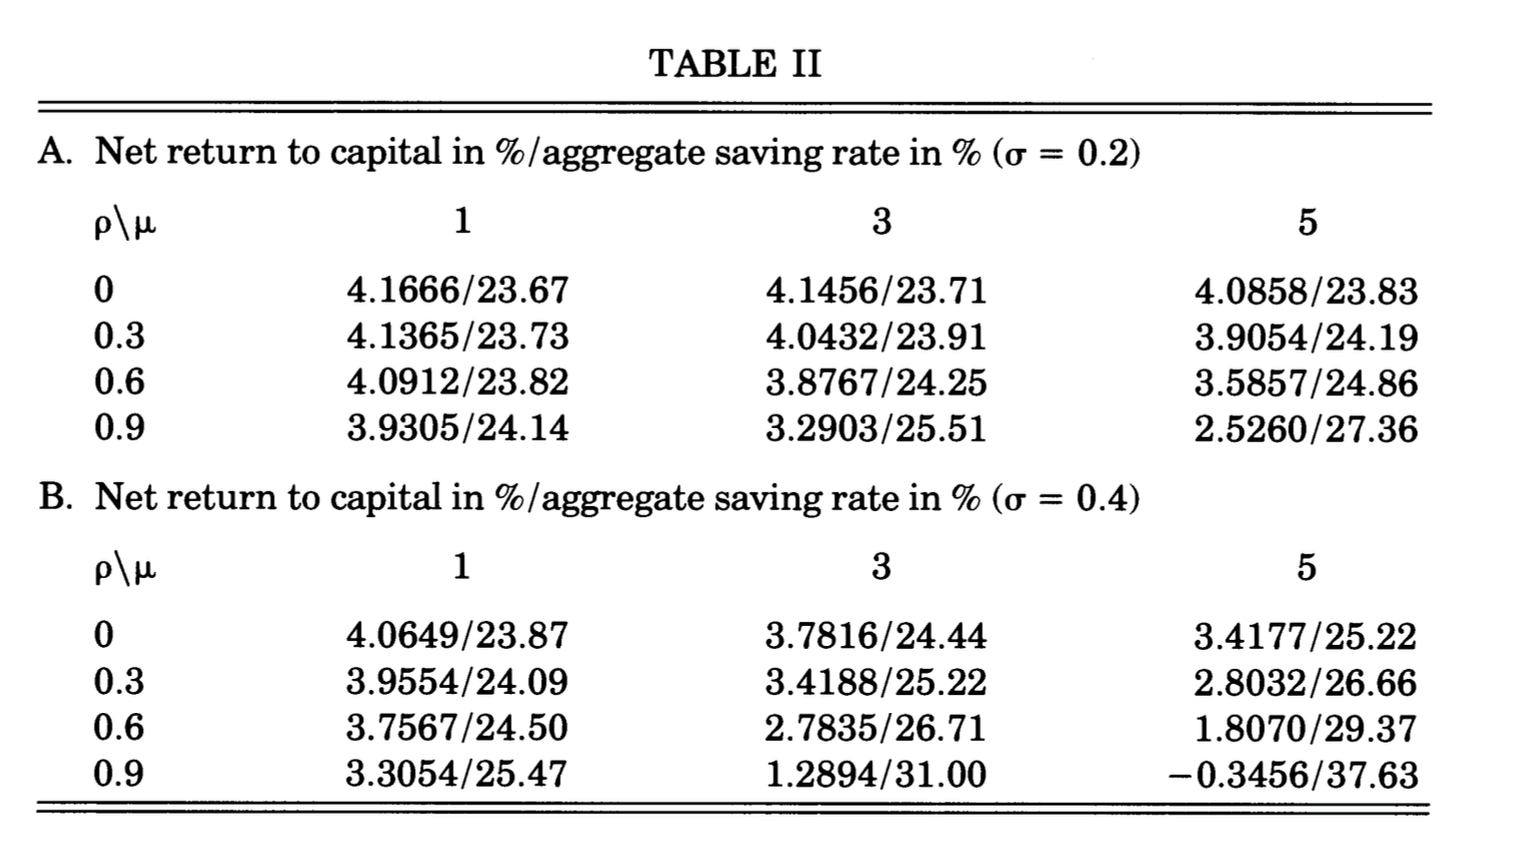
\includegraphics[scale=0.5]{Appendix/Table-Aiyagari}
\end{figure}
